% Final standalone research-project document: upload directly to Overleaf.
% Compile twice with pdfLaTeX, or once with Tectonic's automatic reruns.
% Archived model scores are evidence-derived; broader timing evaluation remains planned.
\documentclass[11pt,a4paper]{article}
\usepackage[T1]{fontenc}
\usepackage[utf8]{inputenc}
\usepackage[margin=0.85in]{geometry}
\usepackage{amsmath,amssymb,booktabs,array,tabularx,longtable}
\usepackage{pdflscape}
\usepackage{tikz}
\usetikzlibrary{arrows.meta,positioning}
\usepackage{enumitem}
\usepackage[hidelinks]{hyperref}
\usepackage{microtype}
\setlist{itemsep=3pt,topsep=5pt}
\setlength{\emergencystretch}{3em}
\renewcommand{\arraystretch}{1.2}
\newcommand{\code}[1]{\nolinkurl{#1}}
\newcolumntype{L}[1]{>{\raggedright\arraybackslash}p{#1}}

\title{\textbf{Predictive Deadline Management with Monitored Recovery for Distributed Edge AI Workflows}\\[0.6em]
\large Real-Time Systems Research Project}
\author{Mayur Raju (24BCS073) \quad P Gnandeep (24BCS095)\\
P Maruthi (24BCS098) \quad P Sanjay (24BCS100)\\
S Sudharsan Reddy (24BCS130)\\[0.5em]
Department of Computer Science and Engineering\\
Course: Real-Time Systems}
\date{12 October 2026}

\begin{document}
\maketitle
\begin{abstract}
Distributed edge devices increasingly execute dependent AI and control workloads
on shared processors, accelerators, and communication links. A computation may
be correct yet arrive too late to be useful. Local contention, thermal slowdown,
remote queueing, and unreliable result delivery make a placement decision based
only on current average latency insufficient. This project investigates a
runtime controller combining graph-based deadline-risk prediction, cooperative
offloading, continuous supervision of remote attempts, and conditionally
admitted local early-exit recovery. A discrete-event research prototype represents
work and time using integer microseconds and records canonical events for
reproducible comparisons. Its learning components execute actual neural
inference and federated updates, while resource service and communication remain
configured simulation models. The evaluation protocol examines deadline misses,
prediction calibration, recovery effectiveness, output-utility proxies, and
protection overhead. The intended contribution is an auditable integration and
evaluation of these mechanisms, rather than a new claim to invent offloading,
early exit, federated learning, or response-time analysis. Expected timing benefits remain hypotheses. This report documents an implemented
prototype, a reproducible recheck of an archived predictor evaluation, and a
protocol for broader timing experiments. Software consistency checks do not
establish universal correctness or physical-system safety.
\end{abstract}

\paragraph{Report scope.}
PredictiveRuntime is an implemented, finite paired simulation prototype for a
Real-Time Systems course project. The report separates current software behavior,
recomputed archived model evidence, and planned research evaluation. It retains
exactly three primary references. Archived timing studies preserve their original
source and model identities and are not presented as newly regenerated results.

\setcounter{tocdepth}{1}\newpage\tableofcontents
\newpage

\section{Problem Statement}
\subsection{Application context}
A drone, mobile robot, or industrial edge device may repeatedly perform sensing,
perception, planning, and actuation alongside telemetry and control tasks.
These stages share CPU, GPU, memory, and radio resources. Their dependencies
form a directed acyclic graph (DAG): a planning stage cannot consume an output
that has not yet been produced by its required predecessors.

Executing everything locally avoids communication but may overload a device.
Offloading can access a faster peer but introduces request serialization,
transport delay, remote waiting, execution, and result return. Conditions may
change after admission. If the controller notices a failure only after the
deadline, even an available local alternative may be useless.

\subsection{Research problem}
The problem is to choose an execution action from information available at the
decision time and supervise that action while a useful recovery opportunity
still exists. The controller must account for its own computational and
communication cost. It must preserve task precedence, avoid duplicate accepted
outputs, and expose unavoidable misses honestly.

The main question is: \emph{Under declared workload, compute, and network models,
when does predictive placement with monitored local recovery reduce workflow
deadline misses, and what additional work and output degradation does it cost?}
This question permits positive, zero, and negative effects.

\subsection{Formal system description}
Let workflow job $J$ have DAG $G_J=(V_J,E_J)$, release time $r_J$, and relative
end-to-end deadline $D_J$. Its absolute deadline is $d_J=r_J+D_J$. Stage $v$
becomes ready at $r_v$ after every required predecessor has committed an output.
Here $r_v$ denotes precedence-ready time, before queue waiting and controller
work. If its relative stage deadline is $D_v$, its absolute deadline is
\begin{equation}
 d_v=\min(r_v+D_v,d_J).
\end{equation}
These readiness-relative stage deadlines are local limits, not a static budget
allocation that guarantees end-to-end feasibility. Placement must also consider
remaining downstream work before $d_J$. A deadline equality counts as timely only
when the valid commitment is processed by that timestamp; simultaneous-event
ordering must be fixed and recorded.

Given the observable state $S(t)$, the controller chooses
\begin{equation}
 a_v(t)\in\{\text{local full execution},\text{eligible peer execution},
 \text{admitted local early exit}\}.
\end{equation}
An exit is eligible only at a declared structural boundary with a valid output
and a remaining-work bound. A fresh local recovery attempt must pay for its own
required prefix; remote progress cannot be reused locally without explicitly
modeled state transfer and compatible checkpoints. A task may have several attempts, but
\begin{equation}
 \sum_{a\in\mathcal A_v}\mathbf 1\{a\text{ commits}\}\leq 1.
\end{equation}
Under the configured firm-deadline drop policy, an unresolved stage or workflow
deadline failure terminates the job's useful execution. Remote cancellation can
still consume work until its delivery or the modeled lease expiry.

\section{Objectives of the Project}
\begin{enumerate}
\item Model heterogeneous devices, dependent workflows, CPU/GPU sharing,
memory admission, thermal derating, and communication failures using a
deterministic discrete-event simulator.
\item Estimate stage deadline-miss risk from a recorded graph of workload and
resource state using a graph neural network, and assess its calibration on
independent evaluation runs.
\item Estimate peer execution latency using decentralized observations and
sample-weighted federated updates, including their modeled resource cost.
\item Select local, remote, or declared degraded execution using remaining
time, feasibility estimates, and output-utility information.
\item Monitor offloaded attempts and admit local recovery before its feasible
window closes, while conserving cancellation work and enforcing one commitment.
\item Produce conditional timing certificates only for supported scheduler
and workload assumptions.
\item Compare executable policies and component ablations using paired seeds,
uncertainty intervals, regressions, overhead, and utility trade-offs.
\item Provide a professional inspection dashboard whose displayed states and
metrics derive from canonical events and matching run manifests.
\end{enumerate}

\section{Operation of the Research Prototype}
\subsection{Execution and observation}
Each configured device hosts repeated workflow jobs. Source stages become ready
at release; successors become ready after committed predecessor results.
Execution demand is sampled from a declared bounded distribution. CPU work is
preemptive under the selected policy; GPU work progresses through modeled layer
boundaries. Memory allocation and sender-radio serialization constrain admission.
Simulation time, work, and service residuals use integers to avoid cumulative
floating-point clock error. Actual full execution demand is sampled for resource
service. The predictor observes the declared WCET budget minus recorded delivered
work, clamped at zero; it does not receive the future sampled demand.

The current interactive model provides one preemptive CPU slot and one GPU slot
per device. GPU interruption occurs at four layer boundaries. CPU and GPU task
memory is fixed at 32 and 128 MiB respectively; GPU ownership also reserves a
configured fraction of CPU service. Periodic workflows are replicated across
configured devices on a complete directed communication mesh. Sporadic releases,
arbitrary sparse routes, configurable stage memory, and physical robot dynamics
are future extensions rather than present features.

Every material transition emits a canonical record with sequence number,
timestamp, device, job, task, attempt, and payload. Separate reducers produce
metrics and dashboard snapshots. The UI cannot create successful execution or
recovery by drawing an animation: a filled milestone requires its recorded event.

\subsection{Prediction and placement}
The graph predictor uses workload and resource relationships to estimate failure
risk; graph encoders of this kind are already used for dependent-task
offloading\cite{chen2026,kaur2025}. Its output is a prediction, not a schedulability certificate. A local
deadline guard and downstream workflow pressure complement the neural threshold.
Candidate peers are checked for estimated completion time, communication cost,
memory, and delivery reliability. The remote estimator targets active execution service duration and on-time
execution reliability; its recorded duration excludes request/result transport
and time spent without a compute slot. Queue and transport terms must therefore
be modeled separately. Its initial latency multiplier is an inherited heuristic,
not demonstrated percentile coverage for current scenarios or online updates.

A useful completion estimate has the form
\begin{equation}
 \widehat T_{\mathrm{remote}}=
 \widehat Q_{\mathrm{sender}}+\widehat T_{\mathrm{request}}+
 \widehat Q_{\mathrm{peer}}+\widehat C_{\mathrm{peer}}+
 \widehat T_{\mathrm{return}}.
\end{equation}
Admission requires this estimate plus charged decision work and a configured
margin to fit the remaining slack. A learned estimate remains a prediction.
In particular, summing component 95th-percentile estimates does not generally
produce a 95th-percentile end-to-end bound. Planned tail evaluation must calibrate
the complete sum, or allocate component failure probabilities with an explicit
combined coverage argument. Feasibility under an estimated state does not
guarantee future completion.

\subsection{Current action-selection rule}
The controller first charges modeled decision work. Neural risk, local stage
slack, and a downstream-work pressure guard determine whether to consider
protection. For an offloadable stage at initial admission, it chooses the
feasible peer with the smallest estimated completion time, using a deterministic
tie-break. If no peer is feasible, it selects the highest configured-utility
eligible exit whose matching fallback certificate passes. Otherwise it continues
local full execution. Checkpoint continuation and predictor-failure behavior
are explicitly recorded.

This is an implemented policy rule, not a proven global utility optimum. Peer
admission checks stage deadlines; the downstream pressure guard does not certify
end-to-end feasibility. A broader utility-aware optimizer is a possible extension.
The GNN has frozen pretrained weights. Actual online SGD and FedAvg update a
separate peer-estimation MLP, not the risk GNN.

\subsection{Monitored recovery}
A watchdog examines remote progress and the local fallback window. Recovery may
be triggered by a worsening completion estimate, a closing local window, or
exhausted delivery retries. A fallback admission check evaluates the declared
remaining work against conservative available service and previously admitted
fallbacks. Unsupported, zero-service, or insufficient-memory cases are rejected.

Recovery does not assume instantaneous peer termination. A cancellation request
is distinct from acknowledgment. Remote work remains charged until it stops,
and an obsolete returned result is discarded. A local accepted output is also
distinct from workflow success: successors can still miss their deadlines.

\subsection{Early exit and output meaning}
The prototype executes a synthetic prefix/full classifier to inspect output
validity and commitment. Declared utility values describe configured trade-offs.
They are not measured perception accuracy. A future application extension would
need a real early-exit model, representative data, and a task-quality metric.
The timing experiment and a future semantic-quality experiment should remain
separate until their model and dataset bindings are explicit.

\section{Literature Review}
This focused review retains exactly three recent primary papers, selected for
direct relevance to dependency-aware deadlines, graph-based federated learning,
and early-exit offloading. Bibliographic identities were checked against publisher
records and author repositories. HiDeR-GQ's accessible accepted manuscript was
also inspected; the other comparisons use publisher or author abstracts and
publication metadata. Those limited comparisons cannot establish that a paper
lacks an unmentioned mechanism. This is not an exhaustive novelty review.

\subsection{Dependency-aware graph offloading and deadline violations}
Chen and colleagues propose FEDG graph features and DGMA multi-agent deep
reinforcement learning for dependency-aware offloading and resource
allocation under partial observability\cite{chen2026}. Adaptive prioritized
replay and selective parameter sharing support collaborative learning.
Their simulated evaluation includes delay, energy, offloading utility, and
deadline violation rate. Thus graph-based offloading evaluated against
deadlines is already established. The proposed study asks a narrower question
about supervising placed attempts and admitting local recovery with explicit
cost and commitment accounting; it does not claim novelty for deadline-aware
graph offloading itself.

\subsection{Graph attention with federated learning: HiDeR-GQ}
Kaur, Cheng, and Kourtessis combine quantized GATv2, personalized federated
DDQN, and latency-aware dependency pruning in HiDeR-GQ\cite{kaur2025}.
The accepted manuscript evaluates simulated DAG workloads, completion delay,
model communication overhead, and deadline violations (Section V-G).
It is therefore a direct precedent for graph-plus-federated deadline-aware
offloading. Here the federated model estimates peer execution rather than
learning an offloading policy. Required workflow edges remain enforced;
removing a dependency would require a separately declared semantic alternative.
Monitored recovery and cancellation accounting are proposed study mechanisms,
not features proved absent from HiDeR-GQ by this review.

\subsection{Joint offloading and early-exit selection}
Angelucci and colleagues jointly optimize offloading, resource allocation,
and early-exit selection using distributional Soft Actor-Critic for edge
inference in a connected-vehicle setting\cite{angelucci2026}.
Their system model includes varying wireless and resource conditions,
and their simulation studies inference accuracy--latency trade-offs and
task completion. This directly establishes prior work on combining early
exit with offloading. The present prototype uses configured utility and
synthetic output checks, so it cannot claim equivalent application-accuracy
evidence. Its proposed comparison concerns workflow deadlines and recovery
after remote admission, rather than an invention of joint exit/offload selection.

\subsection{Selection and scope}
The three papers jointly cover the closest mechanisms under the current
reference limit. Their reported performance belongs to their own experiments;
no percentage is transferred to this project or treated as a matched benchmark.
Standard aggregation, calibration, and timing-analysis equations below specify
the proposed methods and are not claimed as new derivations. A later full paper
should add foundational method citations when the reference limit is relaxed.

\begin{landscape}
\section{Comparison of Related and Existing Works}
\small
\begin{longtable}{L{2.6cm}L{4.0cm}L{4.2cm}L{4.0cm}L{6.0cm}}
\caption{Focused comparison. Evaluation settings belong to the cited papers;
they are not datasets used by this project. No prior system has been reproduced
here.}\label{tab:literature}\\
\toprule
Work & Technique & Evaluation aspects & Evidence setting & Relationship to this study\\
\midrule\endfirsthead
\toprule Work & Technique & Evaluation aspects & Evidence setting & Relationship to this study\\
\midrule\endhead
\bottomrule\endfoot
Chen et al. (2026)\cite{chen2026} & FEDG dependency-aware graph features; DGMA collaborative multi-agent DRL & Delay, energy, offloading utility, deadline violations & MEC simulation; publisher abstract inspected & Prior deadline-aware graph offloading. Proposed addition to evaluate: post-placement recovery and attempt accounting.\\
HiDeR-GQ (2025)\cite{kaur2025} & Quantized GATv2, personalized federated DDQN, dependency pruning & Completion delay, model communication, deadline violations & Simulated DAG workloads; accepted manuscript inspected & Prior graph/federated combination. Our learning target is peer execution; required DAG edges remain enforced.\\
Angelucci et al. (2026)\cite{angelucci2026} & Distributional SAC; joint offload/resource/exit selection & Accuracy--latency trade-off; task completion & Edge-inference simulation for connected vehicles; abstract inspected & Prior early-exit/offload integration. Our current utility is a configured proxy; recovery is evaluated separately.\\
Proposed project & Risk prediction, federated peer estimation, watchdog, conditional local recovery & Workflow and critical-stage misses, calibration, on-time utility, charged cost & Python event simulation; actual neural computation; provenance-bound traces & Auditable integration study; superiority and first-in-field novelty remain unestablished.\\
\end{longtable}
\end{landscape}

\section{Comparison with the Proposed Work and Research Gap}
\subsection{What existing work already establishes}
The selected literature already addresses graph-based dependency handling,
deadline violations, federated offloading policies, and joint early-exit/offload
selection\cite{chen2026,kaur2025,angelucci2026}. Combining named learning
components or changing the objective to deadlines alone is insufficient to
establish a research contribution.

\subsection{The question investigated here}
The proposed study evaluates \emph{prediction before placement with monitored,
conditionally admitted local recovery after placement} for dependent workloads
sharing heterogeneous resources. It records the recovery window, controller
work, network failures, cancellation delay, duplicate-attempt work, and the
single accepted result in one event ledger. This is a scoped experimental
question, not a demonstrated omission across the field.

Does prediction leave enough intervention time? Does monitoring improve
outcomes after conditions change? Do any gains remain after charging learning,
transfer, and degraded-output costs? These questions require executable
ablations, stress cases, uncertainty estimates, and visible regressions.

\subsection{Contribution boundaries}
The intended contribution is an inspectable execution model and reproducible
evaluation of that recovery lifecycle. Built-in scheduling baselines are not
reproductions of the cited systems. A broader review and faithful, matched
implementations would be needed to establish stronger novelty or performance
claims. The present proposal contains no new empirical results.

\section{Proposed Methodology and Architecture}
\subsection{Architecture}
\begin{figure}[htbp]
\centering
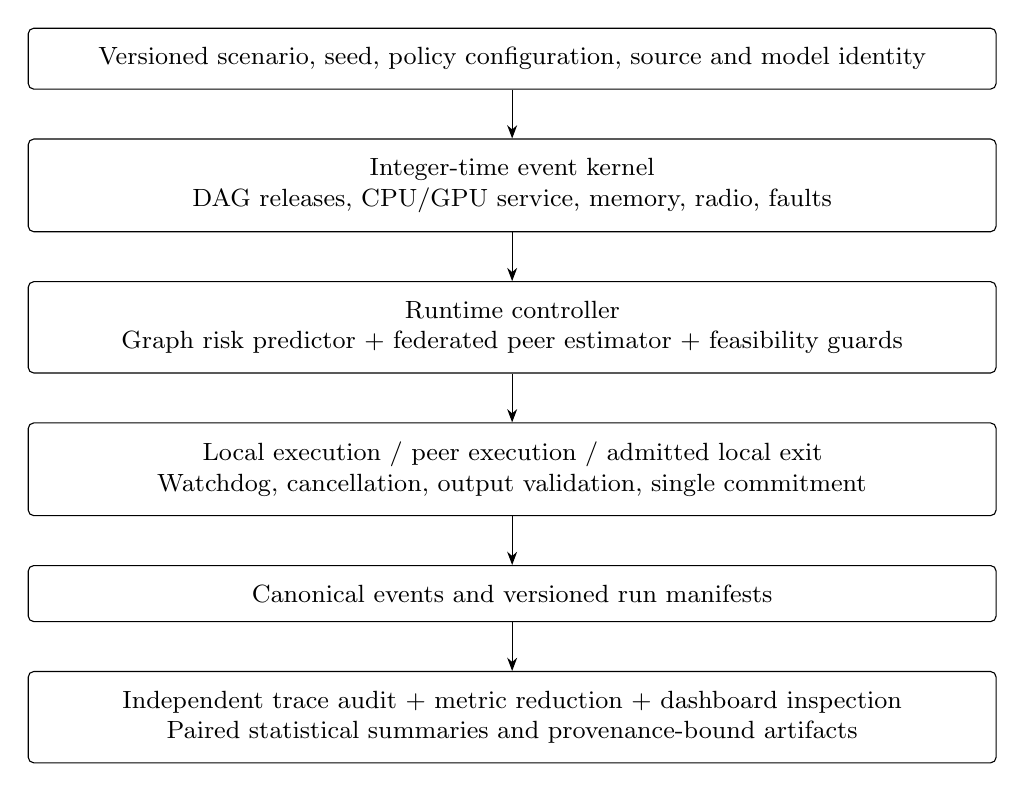
\begin{tikzpicture}[node distance=0.62cm,>=Stealth,
 box/.style={draw,rounded corners=2pt,align=center,text width=11.8cm,
 inner sep=7pt,font=\small}]
\node[box] (spec) {Versioned scenario, seed, policy configuration, source and model identity};
\node[box,below=of spec] (kernel) {Integer-time event kernel\\DAG releases, CPU/GPU service, memory, radio, faults};
\node[box,below=of kernel] (controller) {Runtime controller\\Graph risk predictor + federated peer estimator + feasibility guards};
\node[box,below=of controller] (execution) {Local execution / peer execution / admitted local exit\\Watchdog, cancellation, output validation, single commitment};
\node[box,below=of execution] (events) {Canonical events and versioned run manifests};
\node[box,below=of events] (outputs) {Independent trace audit + metric reduction + dashboard inspection\\Paired statistical summaries and provenance-bound artifacts};
\draw[->] (spec)--(kernel);\draw[->] (kernel)--(controller);
\draw[->] (controller)--(execution);\draw[->] (execution)--(events);
\draw[->] (events)--(outputs);
\end{tikzpicture}
\caption{Research workflow. The controller operates within the event kernel;
the figure separates responsibilities rather than separate physical machines.}
\end{figure}

\subsection{Runtime procedure}
\begin{enumerate}
\item Validate the DAG, hardware, workload bounds, fault windows, and drain horizon.
\item Release a workflow and mark only its source stages ready.
\item Charge the configured decision work and record the observable input graph.
\item Predict risk, estimate local and remote completion, and reject infeasible
candidates. If prediction fails, expose the failure and use the declared fail-safe.
\item Execute the selected action and monitor remote delivery and recovery slack.
\item Admit a declared local exit only when its matching conditional check permits it.
\item Validate the executed output, commit at most one result, and release successors.
\item Resolve misses and drain released jobs before computing final statistics.
\end{enumerate}

\subsection{Communication and service models}
For payload $B$ bytes and bandwidth $b$ bits per second, serialization time is
\begin{equation}
 T_{\mathrm{serialize}}=\left\lceil\frac{8B\cdot10^6}{b}\right\rceil\ \mu\mathrm{s}.
\end{equation}
Queue waiting, base propagation, jitter, retry service, and result return are
separate costs. With independent per-attempt loss probability $p$ and at most
$k$ retries, a single transfer succeeds with probability $1-p^{k+1}$.
This formula depends on the independence assumption and does not model
correlated outages or prove end-to-end task completion.

For service rate $\rho$ in parts per million of reference speed, delivered work
over $\Delta t$ microseconds is calculated with a retained residual $\epsilon$:
\begin{equation}
 w=\left\lfloor\frac{\Delta t\rho+\epsilon}{10^6}\right\rfloor,\qquad
 \epsilon'=(\Delta t\rho+\epsilon)\bmod10^6.
\end{equation}
Service is bounded by remaining work and the current execution boundary.
Thermal/load values are modeled quantities, not hardware measurements.

\subsection{Prediction data and calibration}
The present model uses simulated EDF release-state graphs with labels based on
subsequent observed firm-task failures, including workflow drops. This target is
failure under the no-protection EDF rollout, not a policy-independent probability
of a stage exceeding its own deadline. Drop-induced failures and direct stage
deadline violations must be identified separately. Planned evaluation separates complete
scenario/seed groups before graph sampling. Adjacent states from one rollout
must not cross training and test partitions. Checkpoint states and the
distribution generated by protection require additional evaluation. A reference
risk label at an intervened state requires a matched no-intervention rollout from
that state; a successful protected outcome must not be relabeled as evidence that
the original warning was false. Counterfactual evaluation beyond release-state
rollouts remains planned. Features and normalization must use only information
available at decision time, with normalization fitted on training groups.

For binary label $y_i$ and predicted probability $p_i$, the Brier score is
\begin{equation}
 \mathrm{BS}=\frac1n\sum_{i=1}^n(p_i-y_i)^2.
\end{equation}
For nonempty calibration bins $B_m$, expected calibration error is
\begin{equation}
 \mathrm{ECE}=\sum_m\frac{|B_m|}{n}
 \left|\overline p_{B_m}-\overline y_{B_m}\right|.
\end{equation}
Both depend on the sampled evaluation distribution. Thresholds and positive
temperature parameters are selected using validation data only. AUROC, AUPRC,
recall, calibration, class counts, and useful intervention lead time should be
reported together; a high discrimination score alone does not establish that
recovery can finish on time.

\subsection{Federated estimation}
Federated learning is used in dependency-aware offloading policies\cite{kaur2025};
here it targets peer execution-latency estimation and a separately defined
execution-reliability output. Execution reliability does not include request or
return delivery success unless those outcomes are explicitly part of its label.
At round $q$, participant $k$ trains on $n_k$ eligible local observations and
produces parameters $\theta_k^{(q+1)}$. Sample-weighted aggregation, in the standard Federated Averaging form, is
\begin{equation}
 \theta^{(q+1)}=\sum_{k\in\mathcal K_q}
 \frac{n_k}{\sum_{j\in\mathcal K_q}n_j}\theta_k^{(q+1)}.
\end{equation}
Only successfully delivered updates enter the participant set. Aborted or
otherwise censored observations must not be treated as completed latency
samples. Training only on completed attempts can underrepresent slow peers;
record censoring and assess this selection bias. Reliability needs explicit
eligible success/failure labels rather than completion samples alone. Sample
weights must count actual eligible observations and an empty participant set
must produce no model update. Federated aggregation alone does not guarantee
privacy or robustness to malicious updates. Publication should be atomic and recorded with the model version and
checksum. Validation must examine latency-tail error, reliability estimation,
staleness, and the cost of training and communication.

\subsection{Conditional timing analysis}
For a supported fully preemptive, fixed-priority, single-processor partition with
constrained deadlines, a declared model uses the standard response-time
recurrence
\begin{align}
 R_i^{(0)} &= C_i+B_i+O_i,\\
 R_i^{(m+1)} &= C_i+B_i+O_i+
 \sum_{j\in hp(i)}\left\lceil\frac{R_i^{(m)}+J_j}{T_j}\right\rceil(C_j+O_j).
\end{align}
Here $C_i$ is the declared execution bound, $B_i$ a validated blocking bound,
$O_i$ per-job overhead, $J_j$ higher-priority release jitter, and $T_j$ period or
minimum inter-arrival time. Deadlines are relative to actual release. A matching
certificate requires convergence with $R_i\leq D_i$ for every active task.
An iteration limit is inconclusive; a contradicted assumption is unsupported.
Failure of this conservative test means that schedulability was not established
under the declared model; it is not automatically a witnessed execution miss.
The jitter, blocking, and overhead terms are an explicit model extension and do
not claim that classical response-time analysis proves the dynamic
CPU/GPU/offload scheduler.

The runtime's fallback check is a separate finite-job analysis for an enforced
FIFO fallback lane. It includes own remaining work, earlier admitted fallback
work, conservative GPU blocking where applicable, minimum service, memory, and
margin. Its certificate applies to the particular stage and admission state. The minimum
service calculation uses the configured fault envelope and thermal floor, not
an unobserved guarantee about future hardware behavior.
Neither check certifies the complete dynamic EDF/GPU/network system or a robot's
physical behavior. Measured host inference maxima are not proven WCET bounds.

\section{Software, Tools, Frameworks, Datasets, and Platforms}
\begin{table}[htbp]
\centering\small
\begin{tabularx}{\textwidth}{L{3.2cm}X}
\toprule Component & Selected platform and intended use\\\midrule
Simulation & Python; integer microsecond event clock; immutable scenario specifications; named seeded random streams.\\
Learning & PyTorch and PyTorch Geometric for actual graph inference; local SGD and federated peer-estimator updates.\\
Service/API & FastAPI and Uvicorn for validated scenario, session, step, inspection, and evidence endpoints.\\
Dashboard & HTML, CSS, JavaScript, and SVG; white engineering workbench; keyboard navigation and responsive inspection.\\
Evaluation & NumPy/statistical helpers, Matplotlib, pytest, and Playwright for paired analysis, data-derived figures, behavioral tests, and browser checks.\\
Artifacts & Canonical JSON/JSONL, SHA-256 manifests, archived source/model snapshots, CSV summaries, and standalone LaTeX.\\
Primary data & Simulator-generated labeled runtime traces with scenario, seed, model, and source provenance; not a downloaded hardware benchmark.\\
Optional future data & MNIST or CIFAR-10 for a separate real early-exit classifier study. Their use is planned, not evidence that present utility measures accuracy.\\
Future hardware & Representative edge boards and measured compute/network traces, subject to access; physical validation is outside the present simulation scope.\\
\bottomrule
\end{tabularx}
\caption{Present software choices and explicitly separated future extensions.}
\end{table}

\section{Implementation and Inspection}
\begin{table}[htbp]
\centering\small
\begin{tabularx}{\textwidth}{L{3.0cm}X}
\toprule Responsibility & Current implementation and boundary\\\midrule
Specifications & \code{rts_predictive/domain/}; immutable workload/device specifications, IDs and schema versions.\\
Execution & \code{simulator/research_engine.py}; integer-time releases, precedence, service, transfers, watchdogs and single commitment.\\
Learning & \code{predictors/research_adapter.py}; actual graph inference, integrity-checked bundles, private observations, SGD and atomic federated publication.\\
Analysis & \code{verification/}; separate fixed-priority reference and enforced finite-job fallback certificates, each with its own assumptions.\\
Evidence & \code{dashboard/research_projection.py}, canonical JSONL writers and run manifests; detached snapshots and independently audited records.\\
Application & \code{api/research.py} and \code{frontend/}; finite paired runs, authored scenarios, real 1-ms stepping and keyboard-operable inspection.\\
\bottomrule
\end{tabularx}
\caption{Implementation responsibilities; paths inside the project package are abbreviated.}
\end{table}

The main dashboard displays a finite paired experiment. An older continuous
console and authored demonstration helpers are separate legacy paths; they are
not the same full research pipeline and are excluded from this report's evidence.
Four executable component flags cover watchdog, federated learning, offload,
and fallback. Heuristic-predictor, calibration, reliability-filter, and staleness
ablations remain planned.

\subsection{Reading the simulation}
The Overview guide explains the current release, drain, or complete phase and
the recorded protected-workflow activity. Device cards show occupied CPU/GPU
capacity, including interference; those bars are not task-completion percentages.
Traffic symbols distinguish requests, results, cancellations, and learning updates.
Pause holds the simulation clock, while Step 1 ms advances the actual engine by
1000 microseconds. Inspection and diagram pan/zoom do not advance time.

Tasks and resources show precedence, running allocation, queues, memory, layer
service, and stage deadlines. Runtime protection shows the selected task's exact
prediction and attempt lifecycle. Models and learning separates the frozen GNN
from the online MLP and displays recorded local losses and published versions.
Results retains rescued and regressed paired jobs, provisional denominators,
undefined relative changes at a zero baseline, and final evidence downloads.
Utility is explicitly labeled as a proxy among committed stages.

\section{Evaluation Plan}
\subsection{Scenarios and comparators}
Evaluate nominal load, bursty interference, thermal derating, and unreliable
communication separately. Common random inputs must match releases, task demands, and exogenous faults
across policies. Sharing a seed alone is insufficient when policy-specific
branches consume random draws differently: use streams or draws keyed by
scenario, job, stage, and event role. Extra recovery attempts remain extra work,
and endogenous queue/thermal states may legitimately differ. Compare FIFO,
rate-monotonic priority, EDF, unconditional offload, reactive degradation,
predictive placement without fallback, and the complete policy. These names
describe implemented comparators whose exact dispatch/preemption rules must be
documented; textbook optimality theorems do not automatically apply to this model.

\subsection{Metrics and uncertainty}
The current paired API and study tooling use workflow deadline-miss ratio as
the primary endpoint; this report adopts that definition. The earlier implementation
plan emphasized critical-task misses, so the change in emphasis is disclosed
rather than retroactively changing historical studies. Report critical-stage
outcomes as secondary measures using fixed scenario-defined criticality. Current
ready-task ratios have policy-dependent denominators because early workflow drops
can prevent successor readiness; compare direct misses, drop-induced failures,
and skipped planned stages separately. Choose the principal comparator using
validation data, then freeze it before test evaluation.

For $N$ released jobs and $M$ final missed jobs,
\begin{equation}
 \mathrm{DMR}=M/N,\qquad N>0.
\end{equation}
Report no ratio when the denominator is zero. Interim dashboard denominators
include active released jobs and are provisional. Final values follow the drain. A workflow counts as failed when its useful
execution is terminated by the firm-drop policy or it lacks all required timely
outputs at $d_J$. Report those reasons separately. If a drain horizon leaves
unresolved jobs, mark the run incomplete and report their count; do not silently
exclude them from a final success denominator.
For paired seed $s$, define an improvement in percentage points as
\begin{equation}
 \Delta_s=100(\mathrm{DMR}_{\mathrm{baseline},s}
                  -\mathrm{DMR}_{\mathrm{protected},s}).
\end{equation}
A positive $\Delta_s$ means fewer misses with protection. A dashboard displaying
the signed change in miss rate uses the opposite sign; the convention must be
stated. Relative reduction is undefined for a zero baseline.

Use independent runs as resampling units for paired bootstrap intervals; do
not resample correlated task events as independent replications. Start with at
least 30 paired seeds per principal cell or justify a different count through
precision analysis. Preserve family separation, report negative seeds, and
declare any multiple-comparison procedure before final evaluation.

Planned secondary metrics include critical-stage misses, response-time quantiles,
deadline lateness, recovery and offload rates, configured utility, controller
work, learning work, charged transfer bytes, and wasted remote service. Host
inference samples are measured separately from configured simulation work.
The present reducer reports response mean and observed maximum over committed
stages. Its pooled maximum-minus-minimum field is a heterogeneous response spread,
not release jitter or per-task-type response jitter. An observed maximum is not
an analytical worst-case response-time bound. Quantiles and per-type variability
require explicit reduction from the raw trace.
A planned extension will compute on-time utility per released job with zero
for failed jobs, alongside
utility among successful jobs; the latter alone hides drops. Response-time
quantiles over completed jobs exclude failures and must state that denominator.
A dropped job has no observed completion lateness; report failure time and cause
instead of inventing a completion timestamp.
Single-run examples and implementation-check matrices do not establish
general statistical superiority.

\subsection{Ablations, sensitivity, and failure paths}
Disable watchdog, federated estimation, offload, and fallback independently, and
confirm that each option changes executed events. Planned comparisons also
include a simpler risk heuristic and calibration/reliability variants. Vary
inference work, bandwidth, propagation, loss, interference, fleet size, and run
horizon. Longer runs are needed to assess estimator evolution and startup effects.

Check predictor exceptions, late host recommendations, invalid output tensors,
failed result delivery, exhausted retries, unavailable local service, insufficient
memory, cancellation races, and infeasible fallback. Failed checks must remain
visible rather than silently becoming successful execution.

\subsection{Reproducibility and integrity}
Each reported experimental metric must trace to a versioned run manifest and
raw canonical events. Archive the exact configuration, code state, model bundle,
and environment. Independently check readiness causality, exclusive slot service,
memory bounds, radio serialization, cancellation accounting, valid output, one
commitment, and final job resolution. Recompute neural outputs and federated
publications from recorded inputs. Figures and tables must consume audited
records rather than authored numerical examples.

\section{Bounded Evaluation and Validation}
\subsection{Archived predictor evaluation rechecked from raw evidence}
The saved research GNN's original EDF release-state evaluation was recomputed
from its archived float32/int64 graph inputs and observed rollout outcomes.
Dataset and weight checksums, original run manifests, graph digests, and failure
labels were reconciled. Temperature and threshold selection were reproduced
using validation data only; the threshold differs only within a declared
$10^{-12}$ floating-point tolerance. Test metrics use the saved operating point.

\begin{table}[htbp]
\centering\small
\begin{tabular}{lr}
\toprule Metric & Recomputed archived value\\\midrule
Accuracy & 0.9653 \\
Precision & 0.4000 \\
Recall & 0.7143 \\
F1 score & 0.5128 \\
AUROC & 0.9814 \\
Average precision (AUPRC summary) & 0.6564 \\
Brier score & 0.0156 \\
ECE (10 equal-width bins) & 0.0071 \\
\bottomrule
\end{tabular}
\caption{Original held-out predictor evaluation on simulated EDF release-state
labels. These values do not measure protected-policy or hardware performance.}
\end{table}

The test partition contains 1095 graphs from 6 complete
rollouts and 28 positive failure labels. Graphs from one rollout are
correlated; graph count is not the independent replication count. An always-
nonfailure classifier would have accuracy 0.9744, higher than the learned
classifier at its saved threshold, while detecting no failures. The learned
classifier detects 20 failures, misses 8, and raises 30 false-positive warnings.
Accuracy alone therefore does not establish a useful deadline predictor; recall,
precision, calibration, intervention lead time, and runtime cost must be assessed
together.

The failure label includes firm workflow drops. Resource-cause labels are proxies,
and the timing head remains exploratory. This recheck does not retrain the model
or validate calibration at protected decision/checkpoint states, custom scenarios,
or online peer-model publications.

\paragraph{Evidence binding.}
The table is generated from \code{model-score-recheck.json}, linked by hashes
to \code{models/research_gnn.bundle.json} and its original graph dataset.
\code{training-evidence.json} indexes matching original rollout manifests and
raw events. Both review records are under
\code{.validation/hour-review-20261012/}. The original dataset and source archive
remain under \code{.validation/research-training-final/}.

\subsection{Software checks and their scope}
The review checks source syntax, scenario validation, deadline equality,
precedence, resource/work conservation, cancellation, single commitment,
neural tensor replay, federated update replay, completed downloads, and browser
behavior. Fresh policy/ablation and long-horizon runs preserve their own
configuration and model/source manifests. The complete test suite and real
Chrome exercises check failure recovery, responsive layouts, inspection,
pan/zoom, busy-request guards, and honest negative-result presentation.

Session closure now serializes with in-flight steps and rejects a stale request
before it can advance time or write to closed evidence. Regression tests cover
idempotent close and the delete/step race. Training and fleet-configuration annotations
are also checked for resolvability.

Passing these checks establishes consistency for exercised configurations,
not exhaustive correctness, simulator fidelity to hardware, or deadline superiority.
The final review ledger records exact commands, counts, source identities,
file checksums, assumptions, and unresolved research limits. New check traces
are implementation diagnostics rather than a publication-scale timing benchmark.

\begin{table}[htbp]
\centering\small
\begin{tabular}{lr}
\toprule Source-bound review check & Recorded count\\\midrule
Passing repository tests & 430 \\
Paired policy/ablation cases & 48 \\
Audited policy traces & 96 \\
Replayed neural forward passes & 41581 \\
Replayed federated publications & 143 \\
\bottomrule
\end{tabular}
\caption{Software-consistency diagnostics, not statistical performance or
physical-system assurance. Counts are generated from the completed review logs.}
\end{table}

The matrix uses three paired EDF seeds per configured family and one seed per
other comparator or component ablation. Larger independent performance studies
remain planned. The full matrix precedes the final annotation-only fleet import
cleanup; current-source tests and boundary checks cover that cleanup. Each run
retains its actual source identity rather than inheriting a later revision.
The source-bound report is
\code{.validation/hour-review-20261012/final-runtime-matrix/report.json};
the exact pytest command and output are in \code{full-tests-final.txt}.

\section{Expected Research Outcomes}
\begin{enumerate}
\item A functioning and documented simulator that permits repeatable inspection
of dependent workloads and distributed execution attempts.
\item A traceable controller integrating risk prediction, peer estimation,
monitoring, and structurally valid local recovery.
\item Evidence about the operating conditions in which the policy helps, has no
effect, or harms timing, together with utility and overhead trade-offs.
\item Conditional analytical certificates for supported partitions and fallback
admissions, including assumptions and rejected cases.
\item A professional dashboard that explains actual decisions and outcomes
without inventing runtime states or experimental data.
\item A reproducible study package with raw records, provenance, executable
comparators, and publication-ready artifacts derived from audited runs.
\end{enumerate}
The hypothesis is that monitoring and timely local recovery can improve deadline
outcomes in selected stressed regimes. Excessive inference/training cost or poor
prediction may remove that benefit. A negative finding is a valid research
outcome and can identify practical limits on using learned runtime controllers.

\section{Limitations and Study Notes}
The simulator abstracts real accelerator interruption, cache effects, operating
system scheduling, radio correlations, and thermal dynamics. Shared controller
telemetry currently has no modeled transport delay. Configured utility and
synthetic output validity do not establish perception quality or robot-command
validity. The pretrained risk model's supported distribution must be stated for
each scenario; custom workloads require further calibration assessment.

Archived studies and this report should not be merged into an asserted
new result. For this course report, keep the focused three-paper review. Before a full
publication, broaden the novelty and foundational-method review, freeze the final
evaluation protocol, publish portable raw evidence, and rehearse reproduction
in a clean environment.

\section{Conclusion}
PredictiveRuntime connects deadline-risk prediction, peer execution, monitored
recovery, and conditional local admission in a reproducible event-based simulator.
Its real-time contribution is the explicit treatment of precedence, timing windows,
controller interference, cancellation cost, and single-result commitment.
The current evidence supports bounded software consistency and the archived
release-state predictor evaluation. Broader calibrated timing studies and hardware
validation remain necessary before claiming general deadline benefits or deployment
assurance.

\begin{thebibliography}{3}
\bibitem{chen2026}
X. Chen, Y. Bi, J. Zhang, X. Yuan, D. Niyato, L. Zhao, and X. Wang.
\emph{Task Offloading and Resource Optimization Based on Dependency-Aware
Graph and Collaborative Deep Reinforcement Learning in Mobile Edge Computing}.
IEEE Transactions on Mobile Computing, 25(7):10998--11015, July 2026.
\url{https://doi.org/10.1109/TMC.2026.3665729}.

\bibitem{kaur2025}
M. Kaur, H. Cheng, and P. Kourtessis.
\emph{Quantized Graph-Based Personalized DRL for Dependency-Aware Task
Offloading in Heterogeneous Edge Networks}.
IEEE Transactions on Consumer Electronics, 71(3):8626--8640, 2025.
\url{https://doi.org/10.1109/TCE.2025.3598355}.
Accepted manuscript: \url{https://uhra.herts.ac.uk/id/eprint/27072/}.

\bibitem{angelucci2026}
S. Angelucci, R. Valentini, M. Levorato, F. Santucci, and C. F. Chiasserini.
\emph{Distributional Reinforcement Learning for Task Offloading, Resource
Allocation and Early Exit Selection at the Edge}.
Computer Networks, 288:112652, October 2026.
\url{https://doi.org/10.1016/j.comnet.2026.112652}.
Open-access record: \url{https://iris.polito.it/handle/11583/3013915}.
\end{thebibliography}
\end{document}
